% !TeX root = RJwrapper.tex
\title{Working with daily climate model output data in R and the
\pkg{futureheatwaves} package}
\author{by G. Brooke Anderson, Colin Eason, Elizabeth A. Barnes}

\maketitle

\abstract{%
Research on climate change impacts can require extensive processing, to
incorporate output from ensembles of different climate models and
different simulations of each model. This processing can be particularly
extensive when identifying and characterizing extreme events like heat
waves and frost day spells, as these must be processed from model output
with daily time steps and may use identification threholds based on
local distributions (e.g., 98th percentile temperature for that
location). Here, we provide an overview of working with daily climate
model output data in R. Further, we present the \pkg{futureheatwaves}
package, which we developed to ease the process of identifying,
characterizing, and exploring multi-day extreme events in climate model
output. This package takes as input a directory of projection files from
many climate models, identify all heat waves for multiple cities using a
user-specified heat wave definition, and write an output directory of
files with these heat waves and their characteristics (e.g., length,
absolute and relative temperatures). The \pkg{futureheatwaves} package
then allows the user to create custom functions and apply them across
all heat wave files; this functionality can be used either to explore
heat wave patterns (e.g., average length and intensity across different
climate models) or to apply epidemiological estimates to project health
impacts under different scenarios.
}

\section{Introduction}\label{introduction}

Research on climate change impacts can require extensive processing.
This is not only because output files for a single climate model can be
large, but also because of the rising popularity of ensemble techniques
\citep{IPCCch1}, in which, to better characterize uncertainty in
projections, impacts are assessed for multiple climate models, multiple
simulations of each climate model, and multiple climate experiments.
Projections of regional climate change over the next century are subject
to high uncertainty due to three distinct sources: (1) internal climate
variability, i.e.~climate noise, (2) climate model uncertainty, i.e.~the
same forcing can produce a different response in different models and
(3) scenario uncertainty, i.e.~uncertainty in future climate forcings
(e.g. \citet{hawkins2009potential}). One approach for ensuring that
these sources of uncertainty are characterized is to simulate the future
climate many times with multiple models and for multiple future
scenarios.

For example, the Coupled Model Intercomparison Project, phase 5 (CMIP5;
\citet{taylor2012overview}) brought together dozens of major climate
modeling groups around the world to simulate the same future radiative
forcing scenarios, but with their own models. This created an ensemble
of state-of-the-art climate model projections that allow researchers to
study projections and their uncertainties. Most of these modeling groups
additionally performed more than one simulation for each scenario and
model (i.e.~multiple ensemble members), perturbing the initial
conditions by a very tiny amount to quantify uncertainties due to
internal climate variability.

This processing is particularly intensive for smaller time steps, like
daily climate model output. While some climate impacts can be assessed
using climate model output at monthly, seasonal, or yearly time steps,
the impacts of multi-day extreme events must be assessed using output in
daily time steps. Such multi-day extreme events include heat waves, cold
spells, frost day spells, and droughts. The assessment is further
complicated if extreme events are identified based on conditions that
are rare for a certain location (e.g., 98th percentile of local
temperature distribution for identifying heat waves) \citep{IPCCch1}, as
this event definition must be determined at each study location from
climate model output. Further, it is often of interest to create
summaries of multiple characteristics of these extreme events. One
interest, for example, in interpreting climate change scenarios output
is whether frequency of heat waves or warm spells will change, as well
as how certain characteristics of these extreme events (e.g., length,
intensity) will change under different scenarios \citep{IPCCch1}.

We begin this article with an overview of climate model output data,
particularly daily data, for R users. We outline where data from CMIP5
can be obtained as well as how to work with the file format (netCDF)
from R. We overview some R packages that can be useful when working with
this data, as well as aspects of the data (e.g., non-standard calendars)
of which users should be aware when working with daily climate model
output in R.

After this overview, we present the \pkg{futureheatwaves} package. which
we created to aid in identifying and characterizing any type of
multi-day extreme event from daily climate model output (Table
\ref{tab:goals}). Further, this package provides some functionality
particularly useful in identifying and characterizing heat waves
specifically. Quantifying the impacts of heat waves on human health
suffer from additional sources of uncertainty beyond those inherent in
projections of regional changes in surface temperature. These include:
(1) uncertainty in the ability of communities to adapt to changing
temperatures (the adaptation scenario) and (2) uncertainty in the
definition of a heat wave itself. Thus, identifying and characterizing
the impacts of future heat waves in state-of-the-art climate models
requires analyzing hundreds of projections based on combinations of
anthropogenic activity, climate model and ensemble member, adaptation
scenario, and heat wave definition. Such an analysis is non-trivial. For
example, to estimate the possible impacts of heat waves using 32
ensemble members of CMIP5, two forcing scenarios, two different heat
wave definitions, and five progressive assumptions about adaptation to
heat, would require that one identify and characterize heat waves in 640
separate temperature time series for each region of interest.

\begin{table}[t]
\begin{center}
\newcolumntype{L}[1]{>{\raggedright\arraybackslash}p{#1}}
\begin{tabular}{lL{\dimexpr0.8\textwidth-2\tabcolsep\relax}}
\toprule
 & Design goals of the \pkg{futureheatwaves} package \\
\midrule
1 & Make processing of large sets of climate projections more practical for researchers exploring the potential impacts of heat waves and other multi-day extreme events.\\
2 & Speed up processing time by incorporating C++ in event identification.\\
3 & Keep track of the names of climate models, and number of ensemble members processed for each.\\
4 & Not only identify, but also characterize, all extreme events within each climate projection, to allow the exploration of patterns in these characteristics across different projections and also to allow the use of more complex impacts models, including models that include effect modification by event characteristics (e.g., event length, event intensity). For example, this package allows the user to apply a health effects model where risk of mortality is not the same for every heat wave, but rather is modified by heat wave length, intensity, or other measured characteristics.\\
5 & Give users extensive power in customizing the process, including allowing custom event definitions.\\
6 & Allow users to easily explore the extreme events identified within all climate projections by applying custom functions across heat wave data sets from all projections at once.\\
7 & Create output that is in a ``tidy" data format, allowing it to work well with \pkg{ggplot2} for visualization.\\
\bottomrule
\end{tabular}
\end{center}
\caption{Design goals for the \pkg{futureheatwaves} package.}
\label{tab:goals}
\end{table}

The \pkg{futureheatwaves} package automates the process of identifying
and characterizing multi-day extreme events across different ensemble
members of one or more climate models. A variety of different heat wave
definitions have been used to identify heat waves in a time series of
temperature data \citep{smith2013heat}, and the choice of heat wave
definitions can influence both health effect estimates
\citep{chen2015influence, kent2014heat} and projected heat wave trends
\citep{smith2013heat}. Further, other types of extreme events will be
defined differently than heat waves (for example, frost day spells may
be defined as one or more days with temperature at or below \(0^oC\)).
This package therefore allows the user to create and use a custom the
extreme event definition used to identify events in the climate model
output. Finally, this package allows the user to explore the extreme
events identified in the climate model output with a function that can
take a user-defined R function and apply it across all extreme event
files generated for the separate ensemble members.

\section{An overview of climate model output for R
users}\label{an-overview-of-climate-model-output-for-r-users}

\subsection{CMIP5 climate model output
data}\label{cmip5-climate-model-output-data}

For climate impact studies, a top source for climate model output files
is the Coupled Model Intercomparison Project, which is currently in its
fifth phase (CMIP5). Over 20 climate modeling groups have created one or
more climate models which, for this project, are run using standardized
scenarios \citep{taylor2012overview}. The resulting output is uniform
across modeling groups and has a consistent structure, which allows
comparison of simulations from different models \citep{IPCCch9}. For
CMIP5, each group created simulations under several experiments, with
experiments varying in terms of the radiative forcing. This radiative
forcing depends on time-varying model inputs (greenhouse gas emissions
or concentrations, land use changes, etc.), which are specified for each
experiment \citep{taylor2012overview, IPCCch9}. Experiments include
historical experiments (run using forcings consistent with observed and
reconstructed data for 1850--2005), pre-Industrial control experiments,
and experiments of future scenarios of radiative forcing over the 21st
century or longer (e.g., RCP4.5, RCP8.5) \citep{taylor2012overview}.
Some modeling groups created ensembles of output for a specific model
and experiment, in which they ran the experiment multiple times with the
model with very small changes to the initial conditions, resulting in
multiple ensemble members for a single climate model and experiment.
CMIP5 climate model output is created at a number of different time
steps (e.g., daily, monthly, seasonal, yearly) \citep{taylor2010cmip5},
and some variables are reported at multiple depths in the ocean or
atmosphere (e.g., ocean temperature). Here, we will focus on data with a
daily time step for variables reported at a single depth (e.g.,
near-surface air temperature).

The CMIP5 climate model output data is distributed across data nodes at
different climate modeling centers \citep{taylor2012overview}, but can
be accessed centrally at the World Climate Research Programme CMIP5 data
portal at \url{https://pcmdi.llnl.gov/search/cmip5/}. Users must
register before downloading data, and some data are restricted to
non-commercial use. There is a separate file for each combination of
climate model, experiment, modeling realm (e.g., atmosphere, ocean),
variable, time step, and ensemble member
\citep{taylor2012overview, taylor2010cmip5}. For finer time scales, this
output is further split across multiple files for specific year ranges
(e.g., 5 years of output for each file) \citep{taylor2010cmip5}.
Filenames for CMIP5 files can be parsed to generate information about
the output variable, climate model, experiment, and ensemble member for
the simulation \citep{taylor2010cmip5}. Files can be searched and
downloaded through a point-and-click web interface. The data portal also
allows you to generate a specific wget script, which you can use to
download many files at once. A wget script can also be generated through
Earth System Grid Federation's Search RESTful API. Tips on efficiently
searching and downloading the data, including through use of wget
scripts and the search API, are available as user tutorials through the
website of the University of Colorado Boulder's Earth System CoG (e.g.,
\url{https://www.earthsystemcog.org/projects/cog/doc/wget} for a
tutorial on downloading files using wget).

CMIP5 files are saved in Network Common Data Format (netCDF). NetCDF is
a binary file format that allows storage of data representing a regular
array. These climate model output files can be as large as several
gigabytes {[}?{]}. For climate model output at a single depth (e.g.,
near-surface air temperature), the data is a 3-dimensional array, with
dimensions representing time and two metrics of location (e.g., latitude
and longitude) (Figure \ref{fig:netcdfexample}). Global climate models
generate output at regularly-spaced time steps, typically at
regularly-spaced grid points around the world. The latitude and
longitude spacing of grid points vary by climate model, but are
typically 1--2 degrees for atmospheric variables in CMIP5 models
\citep{IPCCch9}. Each data point in the netCDF array gives the modeled
value of the variable (e.g., surface temperature) for a single time
point and location. For CMIP5 climate model output, the location units
are in degrees east and degrees north for longitude and latitude,
respectively. For daily output files, the time unit is in days since a
specified origin date-time (e.g., days since 1850-01-01 00:00:00)
\citep{taylor2010cmip5}. All CMIP5 output files are requred to include
certain metadata \citep{taylor2010cmip5}. This required metadata
includes the experiment, forcing agents input to the model to create the
simulation, time step, institution and institutional contact
information, climate model, and modeling realm \citep{taylor2010cmip5}.
The metadata also must include units for all of the coordinate variables
(e.g., longitude, latitude, time).

\begin{figure}
\begin{center}
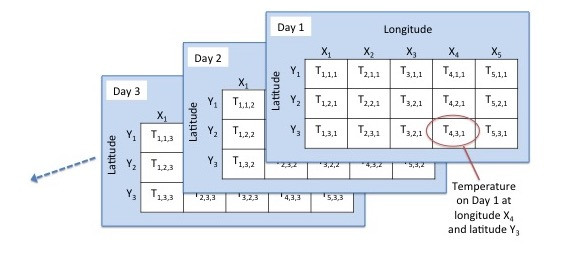
\includegraphics[width = 0.9\textwidth]{netcdf_structure_example}
\end{center}
\caption{Example of structure of a NetCDF climate model output file for a variable reported at a single depth, like surface air temperature. Data are stored in a three-dimensional array, with measurements at each time step and grid location. Surface temperature data are typically indexed in climate model output files by longitude, latitude, and time, in that order. For example, if the air surface temperature ("tas") is read into an R object called \code{tas}, you can access the value for the first day at the fourth longitude and third latitude with \code{tas[4, 3, 1]}. In addition to the output variable (temperature in this example), vectors with the ordered values of each dimension (longitude, latitude, and time) can also be read in from the netCDF file, as well as attribute data (e.g., units for variables, the calendar used for time).}
\label{fig:netcdfexample}
\end{figure}

\citet{taylor2012overview} and \citet{meehl2007wcrp} are excellent
resources for finding out more about the CMIP climate model output data.

\subsection{Working with climate model output in
R}\label{working-with-climate-model-output-in-r}

A few R packages can be used to work with the netCDF file format used
for CMIP5 files. Earlier packages to work with netCDF files included
\pkg{ncdf} and \pkg{ncvar}, but these do not work with the newer netCDF
version 4 released in 2008 and are no longer available through CRAN.
More recent packages, including \pkg{ncdf4} \citep{ncdf4} and
\pkg{RNetCDF} \citep{michna2013rnetcdf, RNetCDF}, work with both version
4 and netCDF's older version 3. Climate model output data for CMIP5 is
required to conform with the earlier version (version 3)
\citep{taylor2010cmip5} and so should work with any of these packages,
although it is safer to write code using functions that can be used with
version for in case future phases of CMIP do not require files to
conform with netCDF version 3.

The netCDF format allows you to access metadata and variables describing
the dimensions of the data without reading the full file into memory.
The metadata describes the dimensions of the array and the units, etc.,
of each variable and is printed by the print method of the R object
returned by the \code{nc\_open} function of \pkg{ncdf4}. For CMIP5
files, the dimension variables include the times and locations
corresponding to each array in the data. Before reading in a variable
from a netCDF file, a connection to the file must be opened, for example
with the \code{nc\_open} function from \pkg{ncdf4}. Variables can then
be read in using the \code{ncvar\_get} function from \pkg{ncdf4}, with
the \code{varid} parameter set to ``lat'', ``lon'', or ``time'' (as a
caveat, many climate models output to non-Gregorian calendars, in which
case the time variable should be read in using a different function, as
discussed later in this section). The climate output variable (e.g.,
near-surface air temperature) can similarly be read in using
\code{ncvar\_get}. In this case, the \code{varid} parameter should be
set using the appropriate CMIP5 variable name (e.g., ``tas'' for
near-surface air temperature); these variable names can be found in the
CMIP Requested Output tables \citep{taylor2010cmip5}. In practice, you
can use the dimensional time and location data to identify the location
of the variable data you need in the netCDF array and use indexing to
read only that data into memory, without needing to read in the full
file \citep{michna2013rnetcdf}. Once the user is done reading in data
from the file, the connection can be closed (e.g., with the
\code{nc\_close} function from \pkg{ncdf4}).

Since the late 1500s, Western dates have been set using the Gregorian
calendar, which has 365.2425-day years. Some climate models, however,
output to different calendars, including the Julian calendar (365.25-day
years), a calendar where there are no leap years (365-day years), a
calendar where every year is a leap year (366-day years), and a calendar
of twelve 30-day months (360-day years) \citep{cfconventions}. With
these non-Gregorian calendars, R's base functions for converting a
vector to a Date class based on the number of days since an origin date
(\code{as.Date}, \code{as.POSIXct}) do not return the desired values.
The \pkg{PCICt} \citep{PCICt} and \pkg{ncdf4.helpers}
\citep{ncdf4.helpers} packages provide further functionality with netCDF
files that can be useful when working with climate model output data and
provide particular help in working with different calendars. CMIP5
netCDF files include information on the calendar used, which the
\code{nc.get.time.series} function in \pkg{ncdf4.helpers} use to convert
the ``time'' variable in the file to an object of the PCICt class, which
provides Date-like functionality for 360- and 365-day calendars
\citep{PCICt}. As a note, while these functions will help with handling
most CMIP5 files, the CMIP5 standards allows use of other calendars
which may not be succesfully handled by these functions, so it is
important to assess whether the time variable range in the PCICt object
correctly matches the expected date ranges for a file as you process
CMIP5 data in R.

The size of the climate model output files can be large enough that it
may make more sense to work with smaller chunks of the data, rather than
reading all data into memory and working with the data all at once
\citep{RCMIP5}. This problem aggregates when working with multiple
climate models and more than one ensemble member for each of those
climate models.

The following code gives an example of using a CMIP5 file and some of
the R packages and functions discussed. Results include a map of
near-surface air temperatures from a single climate model on a specific
date (July 1, 2075) for China (Figure {[}x{]}) and a time series of
daily near-surface air temperature simulations for the climate model
grid point closest to Beijing, China (Figure {[}x{]}). To try this
example, you will need to download the file \ldots{} from \ldots{} and
save it in the ``tmp'' subdirectory of your home directory.

In addition to these general packages for working with netCDF files,
there are several R packages specifically for working with climate model
output data, including \pkg{RCMIP5} \citep{RCMIP5} and \pkg{wux}
\citep{wux}. However, these packages are more useful for working with
data output at time steps of a month or higher and have limited utility
with the daily climate model output data required for studies of
multi-day extreme events.

The \pkg{RCMIP5} package includes functions to read in CMIP5 data from
netCDF files, scan a directory of CMIP5 files and determine models with
continuous available data, create objects of a special ``cmip5data''
class to work with CMIP5 data within R, and parse the filenames for all
files in a directory to extract information within the filename. For
this package, most functions only work with monthly or less frequent
data (e.g., the functions \code{checkTimePeriod} and \code{cmip5data},
as well as functions that work with \code{cmip5data} objects including
\code{filterDimensions} and \code{getProjectionMatrix}) \citep{RCMIP5}.
While the \code{loadCMIP5} function does successfully load the daily
data as a \code{cmip5data} object, most of the methods for this object
type do not do anything meaningful for daily data. The package's
\code{getFileInfo} function, however, will work with CMIP5 files of any
time step; this function identifies all CMIP5 files in a directory and
creates a dataframe that parses the information contained in the file
name. As a note, the \code{get.split.filename.cmip5} function in the
\pkg{ncdf4.helper} package similarly can be used to parse information
contained in CMIP5 file names \citep{ncdf4.helpers}.

The \pkg{wux} package \citep{wux} includes functions that allow the user
to download CMIP5 monthly-aggregated output directly from within R with
the \code{CMIP5fromESGF} function. However, this function does not allow
downloading of climate model output with finer time steps, like daily
data. This package uses the \code{models2wux} function to read in
climate model output netCDF files and convert to a WUX dataframe that
can be used by other functions in the package. While this function can
input climate model output with daily time steps, if the element
``what.timesteps'' of the \code{modelinput} list input is set to
``daily'', the function aggregates this data to a monthly or less
frequent (e.g., seasonal) aggregation when creating the WUX dataframe.
Therefore, while this package provides very useful functionality for
working with averaged output of daily climate model output data, it
cannot easily be used to identify and characterize multi-day extreme
events like heat waves.

More tips on working with CMIP5 files in R are provided in the
``starting\_from\_netcdf'' vignette of the \pkg{futureheatwaves}
package.

\section{\texorpdfstring{The \pkg{futureheatwaves}
package}{The  package}}\label{the-package}

\subsection{How the package works}\label{how-the-package-works}

\begin{widefigure}
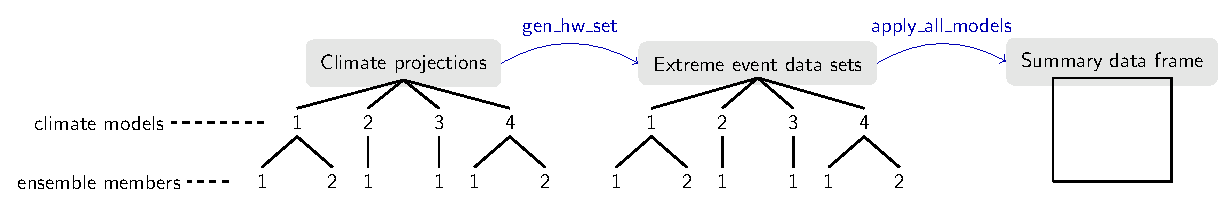
\includegraphics[width = 0.9\textwidth]{OverviewFigure}
\caption{Overview of the functionality of the \pkg{futureheatwaves} package. The package takes a directory with climate projection files (left), for one or more climate models, with one or more ensemble members for each climate model (this example figure shows four climate models with one or two ensemble members each). The gen\_hw\_set function processes these files to create a data frame for each ensemble member, identifying and characterizing all multi-day extreme events (e.g., heat waves) in the time series projection for that ensemble member. The apply\_all\_models function allows users to explore these extreme events by applying user-created functions across all the extreme event data frames, creating a summary data frame with results.}
\label{fig:overview}
\end{widefigure}

The \pkg{futureheatwaves} package was facilitated to aid in identifying,
characterizing, and exploring multi-day extreme events in daily climate
model output data. Figure \ref{fig:overview} gives an overview of the
two primary functions of the \pkg{futureheatwaves} package. First, the
\code{gen\_hw\_set} function processes a directory of climate projection
files that are stored locally on the user's computer (Figure
\ref{fig:overview}, ``Climate projections''), to generate a list of all
extreme events in each projection, as well as over a dozen
characteristics of each identified extreme event (Table
\ref{tab:hwcharacteristics}). The extreme events are identified and
characterized at one or more study locations (e.g., cities), with study
locations specified by the user in an input file. The extreme events
identified for each ensemble member are output as separate files in a
directory specified by the user (Figure \ref{fig:overview}, ``Extreme
events datasets``). Second, the \code{apply\_all\_models} function
allows the user to apply custom functions across all the extreme event
data frames generated by \code{gen\_hw\_set} to summaries of extreme
events across all climate models and ensemble members (Figure
\ref{fig:overview}, right).

\begin{table}
\newcolumntype{L}[1]{>{\raggedright\arraybackslash}p{#1}}
\begin{tabular}{lL{\dimexpr0.8\textwidth-2\tabcolsep\relax}}
\toprule
Column name & Description of characteristic \\
\midrule
\code{mean.var} & Average daily value of the variable across all days in the extreme event, in the units in which the variable is expressed in input files (e.g., average daily mean temperature during the heat wave in degrees Kelvin) \\
\code{max.var} & Highest daily value of the variable across all days in the extreme event, in the units in which the variable is expressed in input files \\
\code{min.var} & Lowest daily value of the variable across all days in the extreme event, in the units in which the variable is expressed in input files \\
\code{length} & Number of days in the event \\
\code{start.date} & Date of the first day of the event \\
\code{end.date} & Date of the last day of the event \\
\code{start.doy} & Day of the year of the first day of the event (1 = Jan. 1, etc.)\\
\code{start.month} & Month in which the event started (1 = January) \\
\code{days.above.abs.thresh.1} & Number of days in the event above a specified absolute threshold (default is the number of days in the event above $80^oF$ / $26.7^oC$, but this can be changed with the \code{absolute\_thresholds} argument in \code{gen\_hw\_set}) \\
\code{days.above.abs.thresh.2} & Number of days in the event above a specified absolute threshold (default is the number of days in the event above $85^oF$ / $29.4^oC$) \\ 
\code{days.above.abs.thresh.3} & Number of days in the event above a specified absolute threshold (default is the number of days in the event above $90^oF$ / $32.3^oC$) \\
\code{days.above.abs.thresh.4} & Number of days in the event above a specified absolute threshold (default is the number of days in the event above $95^oF$ / $35.0^oC$) \\
\code{days.above.99th} & Number of days in the event above the $99^{th}$ percentile of the variable for the location, using the period specified with the \code{referenceBoundaries} argument in \code{gen\_hw\_set} as a reference for determining these percentiles \\
\code{days.above.99.5th} & Number of days in the event above the $99.5^{th}$ percentile of the variable for the location, using the period specified with the \code{referenceBoundaries} argument in \code{gen\_hw\_set} as a reference for determining these percentiles \\
\code{first.in.year} & Whether the event was the first to occur in its calendar year in the location \\
\code{mean.var.quantile} & The percentile of the average variable value during the event compared to the location's year-round distribution of the variable, based on the variable distribution for the location during the period specified by the \code{referenceBoundaries} argument in \code{gen\_hw\_set} \\
\code{max.var.quantile} & The percentile of the maximum variable value during the event compared to the location's year-round distribution of the variable, based on the variable distribution for the location during the period specified by the \code{referenceBoundaries} argument in \code{gen\_hw\_set} \\
\code{min.var.quantile} & The percentile of the minimum variable value during the event compared to the location's year-round distribution of the variable, based on the variable distribution for the location during the period specified by the \code{referenceBoundaries} argument in \code{gen\_hw\_set} \\
\code{mean.seasonal.var} & The location's average seasonal value of the variable (by default, season is set to May--September, but this can be changed with the \code{seasonal\_months} argument in \code{gen\_hw\_set}), based on the variable values for the location during the years specified by the \code{referenceBoundaries} argument in \code{gen\_hw\_set} \\
\code{mean.yearround.var} & The location's average year-round value of the variable, based on the variable values for the location during the years specified by the \code{referenceBoundaries} argument in \code{gen\_hw\_set} \\
\bottomrule
\end{tabular}
\caption{Extreme event characteristics measured by the \code{gen\_hw\_set} function in the \pkg{futureheatwaves} package. The left column gives the name of each variable's column in the extreme event datasets created by the \code{gen\_hw\_set} function. When characterizing extreme events below a threshold, like cold spells, appropriate alternatives are given for some columns (e.g., \code{days.below.abs.thresh.1}, \code{days.below.1st}).}
\label{tab:hwcharacteristics}
\end{table}

The user can extensively customize the definition used to identify
extreme events. The default is a definition for heat waves (two or more
days with temperatures at or above the city's \(98^{th}\) percentile of
year-round temperature), but users can write a custom R function with
either a different heat wave definition or with a definition appropriate
for a different type of extreme event (e.g., one or more days at or
below \(0^oC\) for frost day spells). Some of these heat wave
characteristics are based on relative temperature, which is a measure of
how the temperature during a heat wave compares to the typical
distribution of temperature at that location \citep{IPCCch1}. These
relative temperature metrics will vary depending on whether you
calculate them based on a location's present-day temperature
distribution or on the location's temperature distribution in the
future, since typical temperature distributions in many locations are
expected to change with climate change. The package therefore allows the
user to specify date ranges of the temperature distributions to be used
in calculating these relative temperature metrics in each location.

Second, once the user creates these data frames of location-specific
heat waves, the \texttt{apply\_all\_models} function allows the user to
apply a custom function across all the heat wave data frames that were
generated to create a summary data frame (Figure \ref{fig:overview},
right). This functionality can be used to generate summary statistics
(e.g., determine average heat wave length or total heat wave days), or
can be used to apply more complex functions (e.g., apply epidemiologic
effect estimates across the heat waves to generate health impact
estimates).

\subsection{Example data}\label{example-data}

We have included data files in the package to serve as example files, so
users can try this package before applying it to their own directory of
climate projection files. The example files are all included as
comma-separated (.csv) files, rather than as saved R objects, because
the \texttt{gen\_hw\_set} function requires a directory of
comma-separated files as input and csv is a general file format familiar
to most users. This example data therefore also allow users to see how
to create the appropriate directory set-up for this package.

This example data comes from two climate models that are a part of
CMIP5: (1) the model of the Beijing Climate Center, China Meteorological
Administration (BCC) \citep{xin2013introduction} and (2) the National
Center for Atmospheric Research's (NCAR's) Community Climate System
Model, version 4 (CCSM4) \citep{gent2011community}. We include one
ensemble member from BCC (r1i1p1) and two from CCSM (r1i1p1 and r2i1p1).
To ensure that the size of this example data is reasonably small, we
have only included projection data for grid points from these climate
models that are near five U.S. east coast cities: New York, NY;
Philadelphia, PA; Newark, NJ; Baltimore, MD, and Providence, RI.
Further, to keep the file sizes reasonably small, the historical
projections range over the years 1990 to 1999, while the future
projections are limited to 2060 to 2079. Users' applications of this
package will likely use directories with many more climate model
ensemble members and more locations; however, the operation of the
package is the same for this smaller example application as it would be
for a much larger application.

Once the \pkg{futureheatwaves} package is installed and loaded, the user
can find the local location of these files using R's
\texttt{system.file} function. In the later sections of this article, we
show how to use the package functions with these example files as
inputs.

When setting up to run climate model output data beyond this example
data, any downloaded CMIP5 files will require some pre-processing, in
terms of getting the getting the data into a specific format and storing
these files in a specific directory structure. A file of study locations
must also be saved locally in a specific format. Extensive details on
the required format of files and required input directory structure is
available in the \pkg{futureheatwaves} vignette ``futureheatwaves'',
while tips on processing CMIP5 files into the required structure are
given in the package's ``starting\_from\_netcdf'' vignette.

\subsection{Basic example of processing projection
files}\label{basic-example-of-processing-projection-files}

Once these files and directories are set up, \pkg{futureheatwaves} can
process them to identify and characterize heat waves in each ensemble
member's projection for each location using the \texttt{gen\_hw\_set}
function. For example, to process the example climate projections
directory included with the package, the user can run:

\begin{Schunk}
\begin{Sinput}
projection_dir_location <- system.file("extdata/cmip5",
                                       package = "futureheatwaves")
city_file_location <- system.file("extdata/cities.csv",
                                  package = "futureheatwaves")

gen_hw_set(out = "example_results",
           dataFolder = projection_dir_location ,
           dataDirectories = list("historical" = c(1990, 1999),
                                        "rcp85" = c(2060, 2079)),
           citycsv = city_file_location,
           coordinateFilenames = "latitude_longitude_NorthAmerica_12mo.csv",
           tasFilenames = "tas_NorthAmerica_12mo.csv",
           timeFilenames = "time_NorthAmerica_12mo.csv")
\end{Sinput}
\end{Schunk}

This code first identifies and saves as objects the path names on the
user's computer of the example climate projections directory
(\texttt{projection\_dir\_location}) and the file of study locations
(\texttt{city\_file\_location}). The \texttt{gen\_hw\_set} function
processes this example input and creates a new directory,
\texttt{example\_results}, with files of identified and characterized
heat waves, in the user's current working directory. In this example
code, this processing is done using default values for the heat wave
definition, years for which to generate the heat wave data sets, etc.
Ways to customize these choices are fully explained later in the text.

In this call, the user must specify the directory where the results
should be written (\texttt{out}), the location of the directory of
climate projections (\texttt{dataFolder}), the names of the two main
subdirectories of that climate projection directory, as well as their
year boundaries (\texttt{dataDirectories}; see, for example, Figure
\ref{fig:directories}), the location of the city location file
(\texttt{citycsv}), and the names used for the grid coordinate, climate
projection, and projection date files (\texttt{coordinateFilenames},
\texttt{tasFilenames}, and \texttt{timeFilenames}). When
\texttt{gen\_hw\_set} is run, the user is advised that the function will
write files to his computer and must agree to proceed:

\begin{verbatim}
 Warning: This function will write new files to your computer in the 
 ~/tmp/example_results/ directory of your computer. If that directory already exists,
running this function will write over it. 
 Do you want to continue? (y / n): 
\end{verbatim}

\noindent The function provides status reports while processing. This
helps the user see that the function call is progressing, as
\texttt{gen\_hw\_set} can take a while to run if it is processing many
locations and / or many climate ensemble members. Once the function has
completed running, results will be written locally to the directory
specified by the \texttt{out} argument of \texttt{gen\_hw\_set}. The
structure of this output directory is shown in Figure
\ref{fig:directories} (right). This directory will include files with
some basic information about the climate models and the closest grid
points of each climate model to each location. The output directory will
also include a directory with files of identified and classified heat
waves for each ensemble member, including all characteristics in Table
\ref{tab:hwcharacteristics}.

\subsection{Customizing the extreme event
definition}\label{customizing-the-extreme-event-definition}

The default heat wave definition for this package is:

\begin{quote}
A \dfn{heat wave} is two or more days at or above a city-specific
threshold temperature, with the threshold determined as the \(98^{th}\)
percentile of year-round temperature in the city during some reference
period (by default, 1990--1999).
\end{quote}

Many different definitions of heat waves exist (e.g.,
\citet{smith2013heat, kent2014heat}), so researchers will often want to
use alternative ways to define heat waves. Researchers might want to use
a specific definition, for example, because it matches the definition
used by local health officials to declare heat wave warnings or, in the
case of health impact assessments, to match with a definition used in an
epidemiological study. Three components of the heat wave definition can
be easily customized in the \texttt{gen\_hw\_set} function call, without
creating a new R function to use to identify heat waves. The
customization of the heat wave definition is even more extensive as one
has the option of writing a custom R function.

First, the percentile used to identify a heat wave can be changed using
the \texttt{probThreshold} option in \texttt{gen\_hw\_set}. This option
can take values between 0 and 1. The default value is 0.98, or a
definition with a threshold of the \(98^{th}\) percentile of the
location's temperature. For example, to identify heat waves as two or
more days at or above the city's \(99^{th}\) percentile of year-round
temperature, the user could run:

\begin{Schunk}
\begin{Sinput}
gen_hw_set(out = "example_results",
           dataFolder = projection_dir_location ,
           dataDirectories = list("historical" = c(1990, 1999),
                                        "rcp85" = c(2060, 2079)),
           citycsv = city_file_location,
           coordinateFilenames = "latitude_longitude_NorthAmerica_12mo.csv",
           tasFilenames = "tas_NorthAmerica_12mo.csv",
           timeFilenames = "time_NorthAmerica_12mo.csv",
           probThreshold = 0.99)
\end{Sinput}
\end{Schunk}

\noindent Second, the user can change the number of days used in the
heat wave definition using the \texttt{numDays} argument in the
\texttt{gen\_hw\_set} function. Combined, these two customization
choices can allow the user to identify heat waves using many of the heat
wave definitions used in previous climate and health research-- for
example, 9 of the 16 heat wave definitions used in \citet{kent2014heat}
could be fit using different combinations of these two options for
specifying threshold percentile and number of days.

Third, it is possible to specify the range of years that should be used
when determining this threshold. For example, if you wanted to base the
threshold for each location on its current climate, you could leave this
option as its default, while if you wanted to use a different set of
years (i.e.~a threshold relative to future projected temperatures), you
could set the start and end year bounds for this reference period using
the \texttt{thresholdBoundaries} argument in the function
\texttt{gen\_hw\_set}. For example, to use temperatures in each city
from 2070 to 2079 to determine threshold temperatures, you would run:

\begin{Schunk}
\begin{Sinput}
gen_hw_set(out = "example_results",
           dataFolder = projection_dir_location ,
           dataDirectories = list("historical" = c(1990, 1999),
                                        "rcp85" = c(2060, 2079)),
           citycsv = city_file_location,
           coordinateFilenames = "latitude_longitude_NorthAmerica_12mo.csv",
           tasFilenames = "tas_NorthAmerica_12mo.csv",
           timeFilenames = "time_NorthAmerica_12mo.csv",
           thresholdBoundaries = c(2070, 2079))
\end{Sinput}
\end{Schunk}

It is also possible to use a completely customized heat wave definition.
This functionality allows the user to use heat wave definitions that
either require a number of days above an absolute threshold (e.g.,
maximum temperature of \(\ge95^oF\) for \(\ge1\) day;
\citet{kent2014heat, tan2007heat}) or that require a combination of
thresholds to be met (e.g., maximum daily temperature above a lower
threshold every day of the heat wave and above a higher threshold for a
certain number of days; \citet{kent2014heat, peng2011toward}).

To use a customized heat wave definition, the user can write and load an
R function that implements the definition. To work correctly, this
custom function must allow only specific inputs and generate only
specific outputs. Details about this required structure are provided in
the \pkg{futureheatwaves} package vignette.

To help in developing custom heat wave identification functions, the
package includes an example of the required input data frame,
\texttt{datafr}, which can be loaded with \texttt{data(datafr)}. If a
custom heat wave function is properly set up to use in this package, it
can take as input this example data frame and a threshold value and will
return the original data frame with the columns for whether the day was
part of a heat wave (\texttt{hw}) and, if so, the sequential number of
the heat wave out of all heat waves in that location
(\texttt{hw.number}).

The custom function can then be referenced using the
\texttt{IDheatwavesFunction} option in \texttt{gen\_hw\_set}, and it
will be used to identify heat waves in the data set. As an example, we
have included an alternative ID definition function in this package,
called \texttt{IDHeatwavesAlternative}, which identifies heat waves as
two or more days above the higher of either the location's \(98^{th}\)
percentile temperature or \(80^{o}F\), with the idea that this
definition prevents the identification of heat waves at mild
temperatures in locations with mild or cool climates. The following code
processes the example climate projecting files using this function as
the heat wave definition:

\begin{Schunk}
\begin{Sinput}
gen_hw_set(out = "example_results",
           dataFolder = projection_dir_location ,
           dataDirectories = list("historical" = c(1990, 1999),
                                        "rcp85" = c(2060, 2079)),
           citycsv = city_file_location,
           coordinateFilenames = "latitude_longitude_NorthAmerica_12mo.csv",
           tasFilenames = "tas_NorthAmerica_12mo.csv",
           timeFilenames = "time_NorthAmerica_12mo.csv",
           IDheatwavesFunction = "IDHeatwavesAlternative")
\end{Sinput}
\end{Schunk}

With this ability to write and use a custom heat wave identification
function, most heat wave definitions can be applied with this package.
The exception is definitions that require two separate temperature
metrics (e.g., maximum temperature above a certain threshold or minimum
temperature above a different threshold;
\citet{kent2014heat, robinson2001definition}), because the
\texttt{gen\_hw\_set} function cannot take as input projections of more
than one temperature metric. Definitions that use a heat metric that
combines multiple inputs (e.g., heat index, which is a combined measure
of temperature and air moisture) can be used, but require that the
calculation of the metric is done when creating the input files to
include in the ``Climate projections" directory (Figure
\ref{fig:overview}, left), rather than as part of the heat wave
definition function.

To increase processing speed when identifying heat waves, we coded parts
of the default heat wave identification function in C++ and synced it
with R using the \CRANpkg{Rcpp} package \citep{Rcpp}. Users should
consider a similar strategy for custom heat wave definitions, especially
if processing a large number of climate projection files.

\subsection{Exploring extreme events}\label{exploring-extreme-events}

Once you have created a directory of files with characterized heat waves
for each ensemble member, the results can be explored using the
\texttt{apply\_all\_models} function. This function allows the user to
apply custom R functions across all heat wave data frames created by the
\texttt{gen\_hw\_sets} call. The user can apply any R function that
follows certain standards in accepting input and returning output. Full
details on these standards are given in the \pkg{futureheatwaves}
package vignette.

As an example, if the user wanted to to get the average temperature of
the heat waves identified within each ensemble member, he or she could
write a simple function:

\begin{verbatim}
average_mean_temp <- function(hw_datafr){
        out <- mean(hw_datafr$mean.var)
        return(out)
        }
\end{verbatim}

\noindent The \texttt{apply\_all\_models} function can then apply this
\texttt{average\_mean\_temp} function across the heat wave data frames
for all ensemble members in all climate models:

\begin{Schunk}
\begin{Sinput}
out <- system.file("extdata/example_results", package = "futureheatwaves")
apply_all_models(out = out, FUN = average_mean_temp)
\end{Sinput}
\begin{Soutput}
#>   model ensemble    value
#> 1  bcc1        1 302.3745
#> 2  ccsm        1 302.4458
#> 3  ccsm        2 302.3428
\end{Soutput}
\end{Schunk}

Note that the location of the directory with the heat wave data frames
must be specified using the \texttt{out} argument when calling
\code{apply\_all\_models}. Typically, this will be the directory path
for the directory specified with the \texttt{out} argument in
\code{gen\_hw\_set}. Location-specific results can be generated using
the \code{city\_specific} argument in \code{apply\_all\_models}:

\begin{Schunk}
\begin{Sinput}
apply_all_models(out = out, FUN = average_mean_temp, city_specific = TRUE)
\end{Sinput}
\begin{Soutput}
#>    model ensemble city    value
#> 1   bcc1        1 balt 305.1816
#> 2   bcc1        1  nwk 300.3367
#> 3   bcc1        1   ny 300.3367
#> 4   bcc1        1 phil 305.1816
#> 5   bcc1        1 prov 298.0402
#> 6   ccsm        1 balt 303.1277
#> 7   ccsm        1  nwk 302.4053
#> 8   ccsm        1   ny 302.4053
#> 9   ccsm        1 phil 302.3425
#> 10  ccsm        1 prov 301.8895
#> 11  ccsm        2 balt 302.9373
#> 12  ccsm        2  nwk 302.2748
#> 13  ccsm        2   ny 302.2748
#> 14  ccsm        2 phil 302.2858
#> 15  ccsm        2 prov 301.9520
\end{Soutput}
\end{Schunk}

This output is structured as ``tidy" data \citep{wickham2014tidy},
allowing it to be used easily with the graphing package
\CRANpkg{ggplot2} \citep{ggplot2}.

The \texttt{apply\_all\_models} function can also be used to project the
health impacts of heat waves. As a very simplistic example,
\citet{anderson2009weather} estimated that heat waves, defined as two or
more days at or above a community's \(98^{th}\) percentile temperature,
were associated with an added relative risk of 1.032 for
cardiorespiratory mortality risk in 107 U.S. communities. A simple
estimate of excess deaths associated with this added heat wave risk in a
community can be calculated as \citep{peng2011toward}:

\begin{equation}
E_c = N_c * (RR - 1) * L_c 
\label{eq:healthimpacts}
\end{equation}

where:

\begin{itemize}
\tightlist
\item
  \(E_c\) is the total number of excess deaths in community \(c\);
\item
  \(N_c\) is the baseline average daily mortality in community \(c\);
\item
  \(RR\) is the relative risk of cardiorespiratory mortality per day
  associated with a heat wave; and
\item
  \(L_c\) is the total number of heat wave days in community \(c\) over
  the study period.
\end{itemize}

This impact assessment equation can be translated into a function that
merges each projection's heat wave data frame with a data frame of
community-specific baseline mortality rates (\(B_c\)), calculates
equation \ref{eq:healthimpacts} for each heat wave, and then sums up the
total excess deaths across all heat waves:

\begin{verbatim}
excess_deaths <- function(hw_datafr, base_mortality, RR = 1.032){
        hw_datafr <- dplyr::left_join(hw_datafr, base_mortality,
                                      by = "city") %>%
                dplyr::mutate(excess_deaths = base_mort * length * RR)
        out <- sum(hw_datafr$excess_deaths)
        return(out)
}
\end{verbatim}

\noindent Once defined in R, this function can be applied across all
heat waves from all climate models' ensemble members, provided that you
have a data frame called \texttt{city\_mortality} with columns with each
community's identifier (\texttt{city}) and baseline mortality rate
(\texttt{base\_mort}), using the call:

\begin{Schunk}
\begin{Sinput}
apply_all_models(out = out, FUN = excess_deaths, base_mortality = city_mortality)
\end{Sinput}
\end{Schunk}

As examples of the type of functions that can be used with
\texttt{apply\_all\_models}, we have included several simple functions
for exploring heat waves (Table \ref{tab:applyfunctions}). We included
an example data frame representative of the heat wave data frames that
\texttt{gen\_hw\_set} outputs, to use to test new functions. This data
can be loaded with \texttt{data(hw\_datafr)}. The process for creating a
new function to use to explore heatwaves should be to:

\begin{enumerate}
\def\labelenumi{\arabic{enumi}.}
\tightlist
\item
  Load the example data frame with \texttt{load(hw\_datafr)};
\item
  Build a function that works with \texttt{hw\_datafr} as an input; and
\item
  Apply the function with \texttt{apply\_all\_models} to process all of
  the heat wave files.
\end{enumerate}

\begin{table}
\centering
\begin{tabular}{ll}
\toprule
Function & Description \\
\midrule
\code{number\_of\_heatwaves} & Determines the number of extreme events\\
\code{heatwave\_days} & Sums up the total number of extreme event days across all heat waves\\
\code{average\_length} & Calculates the average length of extreme events\\
\code{average\_mean\_temp} & Calculates the average mean temperature across all extreme events\\
\bottomrule
\end{tabular}
\caption{Example functions included in the \pkg{futureheatwaves} package that can be used to explore extreme events using the \code{apply\_all\_models} function.}
\label{tab:applyfunctions}
\end{table}

\subsection{Customizing dates for projections and reference
temperatures}\label{customizing-dates-for-projections-and-reference-temperatures}

By default, the \texttt{gen\_hw\_set} function will generate heat wave
projections for the years 2070 to 2079, to align with the example data.
This projection date range can be changed by specifying alternative
starting and ending years in the \texttt{projectionBoundaries} argument
of the \texttt{gen\_hw\_set} function. For example, to create
projections for 2060 to 2079, the user would call:

\begin{Schunk}
\begin{Sinput}
gen_hw_set(out = "example_results",
           dataFolder = projection_dir_location ,
           dataDirectories = list("historical" = c(1990, 1999),
                                        "rcp85" = c(2060, 2079)),
           citycsv = city_file_location,
           coordinateFilenames = "latitude_longitude_NorthAmerica_12mo.csv",
           tasFilenames = "tas_NorthAmerica_12mo.csv",
           timeFilenames = "time_NorthAmerica_12mo.csv",
           projectionBoundaries = c(2060, 2079))
\end{Sinput}
\end{Schunk}

The heat wave data sets characterize heat wave in several ways that are
based on relative temperature (for example, the
\texttt{mean.temp.quantile}, \texttt{max.temp.quantile}, and
\texttt{min.temp.quantile} columns described in Table
\ref{tab:hwcharacteristics}). These characteristics are measured for
each of the heat waves identified by the \texttt{gen\_hw\_set} function
by taking the absolute temperature of the heat wave (e.g., average
temperature during the heat wave is \(90^oF\)) and comparing it to the
heat wave location's typical temperature distribution. This process
generates relative measures of how intense the heat wave is compared to
what is normal in that location (e.g., \(90^oF\) is in the \(99^{th}\)
percentile of year-round temperatures in the location).

The values of these relative heat wave characteristics will depend on
what time period is used to determine the location's typical temperature
distribution. For example, the same heat wave would likely have much
higher values for these relative characteristics if the temperature
during the heat wave is compared to typical temperatures in the present
day for that location versus if the temperature is compared to typical
temperatures much later in the \(21^{st}\) century for the same
location.

The default in the \texttt{gen\_hw\_set} function is to use temperatures
for the period 2070 to 2079 for these reference temperatures to
calculate all relative heat wave characteristics. However, the user can
change this specification using the \texttt{referenceBoundaries} option
of \texttt{gen\_hw\_set}. This functionality can be useful in exploring
the role of adaptation in future heat waves. For example, to use
temperature projections for 1990 to 1999 when calculating relative
characteristics of heat waves, to explore the assumption that cities
remain adapted to their present-day climate, rather than changing in
adaptation as climate change increases temperatures, a user could run:

\begin{Schunk}
\begin{Sinput}
gen_hw_set(out = "example_results",
           dataFolder = projection_dir_location ,
           dataDirectories = list("historical" = c(1990, 1999),
                                        "rcp85" = c(2060, 2079)),
           citycsv = city_file_location,
           coordinateFilenames = "latitude_longitude_NorthAmerica_12mo.csv",
           tasFilenames = "tas_NorthAmerica_12mo.csv",
           timeFilenames = "time_NorthAmerica_12mo.csv",
           referenceBoundaries = c(1990, 1999))
\end{Sinput}
\end{Schunk}

For these date range specifications, there are some restrictions on
which year ranges can be selected. The starting year cannot be earlier
than the first year in the first subdirectory, the ending year cannot be
later than the last year of the second subdirectory, and the custom date
boundaries cannot span the two subdirectories.

\subsection{Mapping grid points}\label{mapping-grid-points}

It can be useful to explore the location of the climate model grid point
used to pull climate model output for each study location with a given
climate model. Therefore, the package has a function called
\texttt{map\_grid\_leaflet} that plots the locations of grid points used
for each location from each climate model. This function is built using
the htmlWidget \pkg{leaflet} package \citep{leaflet}. The following code
illustrates the use of this function with the example data to create
Figure \ref{fig:gridmap}, which plots the grid points used in the
example data from the BCC climate model in the example data:

\begin{Schunk}
\begin{Sinput}
out <- system.file("extdata/example_results", package = "futureheatwaves")
map_grid_leaflet(plot_model = "bcc1", out = out)
\end{Sinput}
\end{Schunk}

\begin{figure}
\begin{center}
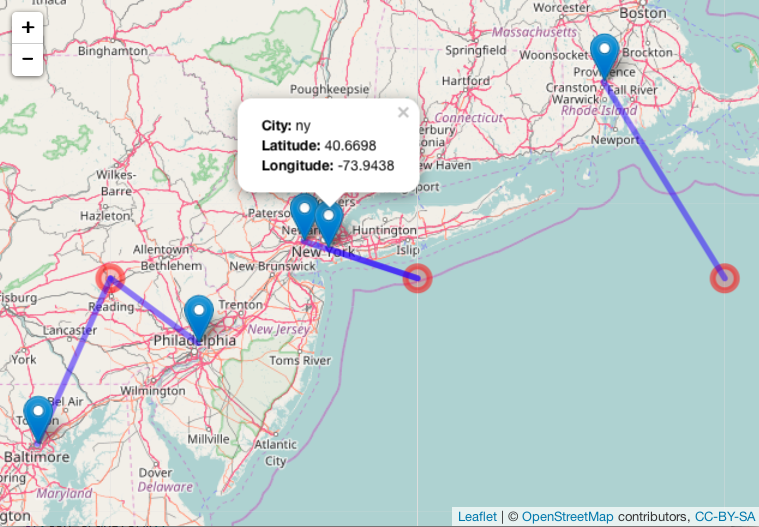
\includegraphics[width = 0.9\textwidth]{ExampleLeaflet}
\end{center}
\caption{Snapshot of an example interactive map created using the \code{map\_grid\_leaflet} showing the locations of study cities and their matching climate model grid points for the BCC climate model example data included with \pkg{futureheatwaves}. The lines on the map connect each climate model grid point to the study location(s) for which that grid point was used. The interactive maps include pop-ups with city identiers; one is shown open in this snapshot as an example.}
\label{fig:gridmap}
\end{figure}

\subsection{Extensions}\label{extensions}

The functionality of this package can be easily expanded by loops. For
example, to explore the role of the heat wave definition on projections,
the user could create a loop to run \texttt{gen\_hw\_set} and
\texttt{apply\_all\_models} to the same directory of climate projections
but with a variety of different functions used to identify the heat
waves in the projections.

Also, while this package was created to be used for research on heat
waves in climate change projections, with some modifications it can be
used more broadly. For example, there are other episodes like wildfires
and air pollution where it may be interesting to identify extended
periods of high exposures in projection time series, and this package
could be applied to explore these exposures. The directory of projection
data would need to be set up in the same structure as for exploring heat
waves, and the \texttt{input\_metric} should be set as
\texttt{fahrenheit}, to pass the exposure values through to the
characterized data sets without performing a conversion. A user could
also use this package to explore events that must be lower than some
minimum threshold (e.g., cold waves), but it would take some extra
coding and conversions, since the functions in this package are written
to identify periods above a threshold (for example, the user could
multiple all projected temperatures by -1, and then the coldest
temperatures would register as being the highest).

\begin{Schunk}
\begin{Sinput}
## Cold wave example
gen_hw_set(out = "example_results",
           dataFolder = projection_dir_location ,
           dataDirectories = list("historical" = c(1990, 1999),
                                  "rcp85" = c(2060, 2079)),
           citycsv = city_file_location,
           coordinateFilenames = "latitude_longitude_NorthAmerica_12mo.csv",
           tasFilenames = "tas_NorthAmerica_12mo.csv",
           timeFilenames = "time_NorthAmerica_12mo.csv", 
           probThreshold = 0.10, 
           above_threshold = FALSE, 
           absolute_thresholds = c(266, 263, 260, 258), 
           seasonal_months = c(12, 1, 2))
\end{Sinput}
\end{Schunk}

\begin{quote}
Extreme statistics and spell-lengths: ``A `frost day' is defined as one
during which the minimum temperature falls below freezing point (0
degC). This is described as a climatological statistic, in which the
minimum temperature is first calculated within each day, and then the
number of days or spell lengths meeting the specified condition are
evaluated.'' (from one example in
\url{http://cfconventions.org/Data/cf-conventions/cf-conventions-1.6/build/cf-conventions.html\#calendar})
\end{quote}

Users doing these kinds of extensions will need to pay attention to a
few points. First, some of the event characteristics (first in the
calendar year, average of May--September temperatures, days above
\(90^{o}F\)) might not be meaningful for studies of other types of
events. Further, because event periods are usually defined as a string
of multiple days exceeding some threshold, the functions in this package
may miss the first and last event of the time period. For example, if
the first day of the time series is the last day of an event, this
function would not identify that event because it lacks data from the
earlier days that allow this day to meet the event definition. This
issue would lead to, at most, missing two events out of each projection,
but should be considered if studying events that might occur near the
start and end of projection data. If there is adequate interest from
researchers, in the future we may adapt the package to make these
secondary applications part of the package.

\section{Acknowledgements}\label{acknowledgements}

This work was supported by grants from the National Institute of
Environmental Health Sciences (R00ES022631), the National Science
Foundation (1331399), and the Colorado State University Vice President
for Research.

\bibliography{Anderson}

\address{%
G. Brooke Anderson\\
Colorado State University\\
Department of Environmental \& Radiological Health Sciences\\ 1681 Campus Delivery\\ Fort Collins, Colorado 80523\\
}
\href{mailto:brooke.anderson@colostate.edu}{\nolinkurl{brooke.anderson@colostate.edu}}

\address{%
Colin Eason\\
Colorado State University\\
Department of Computer Science\\ 1873 Campus Delivery\\ Fort Collins, Colorado 80523\\
}
\href{mailto:aimesce@gmail.com}{\nolinkurl{aimesce@gmail.com}}

\address{%
Elizabeth A. Barnes\\
Colorado State University\\
Department of Atmospheric Science\\ 1371 Campus Delivery\\ Fort Collins, CO 80523\\
}
\href{mailto:eabarnes@atmos.colostate.edu}{\nolinkurl{eabarnes@atmos.colostate.edu}}

